\chapter{Giới thiệu}
\label{Chapter1}
\graphicspath{{Chapter1/Chapter1Figs}}
\justifying

\setlength{\parindent}{6.5ex}
% Ngôn ngữ để viết và trình bày báo cáo khóa luận tốt nghiệp, đồ án tốt nghiệp, thực tập tốt nghiệp (sau đây gọi chung là báo cáo) là tiếng Việt hoặc tiếng Anh. 
% Trường hợp chọn ngôn ngữ tiếng Anh để viết và trình bày báo cáo,  sinh viên cần có đơn đề nghị, được cán bộ hướng dẫn (CBHD) đồng ý và nộp cho bộ phận Giáo vụ của Khoa vào thời điểm đăng ký đề tài để xin ý kiến.
% Báo cáo viết và trình bày bằng tiếng Anh phải có bản tóm tắt viết bằng tiếng Việt.


%Tóm tắt khóa luận được trình bày nhiều nhất trong 24 trang in trên hai mặt giấy, cỡ chữ Times New Roman 11 của hệ soạn thảo Winword hoặc phần mềm soạn thảo Latex đối với các chuyên ngành thuộc ngành Toán.

%Mật độ chữ bình thường, không được nén hoặc kéo dãn khoảng cách giữa các chữ.
%Chế độ dãn dòng là Exactly 17pt.
%Lề trên, lề dưới, lề trái, lề phải đều là 1.5 cm.
%Các bảng biểu trình bày theo chiều ngang khổ giấy thì đầu bảng là lề trái của trang.
%Tóm tắt luận án phải phản ảnh trung thực kết cấu, bố cục và nội dung của luận án, phải ghi đầy đủ toàn văn kết luận của luận án.
%Mẫu trình bày trang bìa của tóm tắt khóa luận (phụ lục 1).


Hiện nay, với việc bùng nổ dữ liệu trên mạng Internet, người dùng có cơ hội tiếp cận nhiều hơn với đa dạng các sản phẩm trên nền tảng số. Tuy nhiên, do có quá nhiều sản phẩm nên người dùng cũng sẽ gặp khó khăn trong việc tự tìm kiếm các sản phẩm phù hợp với mình; nhà cung cấp sản phẩm cũng sẽ gặp khó khăn về lợi nhuận nếu họ có rất nhiều sản phẩm nhưng chỉ có một số ít được người dùng biết đến.
Hệ thống gợi ý sản phẩm (recommender system) được đưa ra nhằm giải quyết vấn đề này; hệ thống sẽ tự động gợi ý các sản phẩm mà được dự đoán là phù hợp cho từng người dùng. Hiện nay, hệ thống gợi ý đóng vai trò quan trọng đối với nhiều nhà cung cấp sản phẩm. Chẳng hạn, theo số liệu tổng hợp được từ tổ chức Ivy Pro School \cite{ivy}, 38\% lượt click từ người dùng Google đến từ hệ thống gợi ý và 35 sản phẩm được bán trên Amazon thông qua hệ thống gợi ý sản phẩm.

Trong lĩnh vực khoa học máy tính, hệ thống gợi ý sản phẩm là một chủ đề 
đang được quan tâm và nghiên cứu từ cộng đồng nghiên cứu khoa học.
Bài toán xây dựng hệ thống gợi ý được phát biểu như sau:
\begin{itemize}
    \item Đầu vào là lịch sử tương tác của người dùng (user) với các sản phẩm (items) hoặc có thêm các thông tin mô tả của sản phẩm 
    (các sản phẩm ở đây có thể là: quảng cáo, bộ phim, bài hát, sách, ... tùy thuộc vào lĩnh vực cụ thể).
    \item Yêu cầu máy tính tự động đưa ra các sản phẩm (không có trong lịch sử tương tác) được dự đoán là phù hợp với người dùng.
    %Chúng tôi gọi sản phẩm phù hợp với người dùng là sản phẩm được người dùng ``thích''.
\end{itemize}

Tuy vậy, việc xây dựng một hệ thống gợi ý sản phẩm một cách hiệu quả là không đơn giản.
Đầu tiên, bản chất của từng lĩnh vực cụ thể sẽ ảnh hưởng đến khả năng giúp ích của hệ thống gợi ý.
Từ thực tế cho thấy, các lĩnh vực mà sản phẩm ``tiêu thụ'' và ``sản xuất'' nhanh như: phim, hình ảnh, âm nhạc, ... 
thì hệ thống gợi ý sẽ ít nhiều đóng vai trò quan trọng. 
Cũng theo số liệu từ Ivy Pro School \cite{ivy}, 75\% số bộ phim được thuê trên Netflix (một nền tảng chiếu phim trực tuyến lớn nhất hiện nay) thông qua hệ thống gợi ý, chứng tỏ sự ảnh hưởng lớn của hệ thống gợi ý đối với lĩnh vực này. 
Mặt khác, hệ thống gợi ý tác động không nhiều đến các lĩnh vực cung cấp dịch vụ hay sản phẩm giá trị cao như:
thuê nhà, phương tiện giao thông, thiết bị điện tử, ... vì người dùng cần đánh giá thông qua nhiều yếu tố mới có thể quyết định được. 
Thứ hai, tùy thuộc vào nhu cầu của người sử dụng mới có thể lựa chọn cách mà hệ thống gợi ý hoạt động.
Việc gợi ý các sản phẩm phù hợp với người dùng dựa vào nhóm người dùng có sở thích tương tự với họ 
hay cách dựa trên các sản phẩm có liên quan với các sản phẩm mà họ đã ``thích'' trước đó là khác nhau.
Một điều nữa cũng có thể được xem là khó khăn thứ ba khi xây dựng hệ thống gợi ý, cả trong cộng đồng nghiên cứu khoa học cũng như thực tiễn, 
đó là ta cần một độ đo và một phương pháp để đánh giá một cách tổng thể và khách quan nhất, 
khi mà dữ liệu và các thuật toán để xây dựng hệ thống gợi ý là rất đa dạng.

Để xây dựng hệ thống gợi ý, một hướng tiếp cận chúng ta thường nghĩ ngay đến đầu tiên
là dự đoán các sản phẩm có ``độ tương đồng'' cao so với các sản phẩm người dùng đã ``thích'' trước đó;
hướng tiếp cận này được gọi là ``Content-Based Filtering'' (lọc dựa trên nội dung) (hình~\ref{fig_CBF} mô tả hướng tiếp cận này).
\begin{figure}
    \centering
	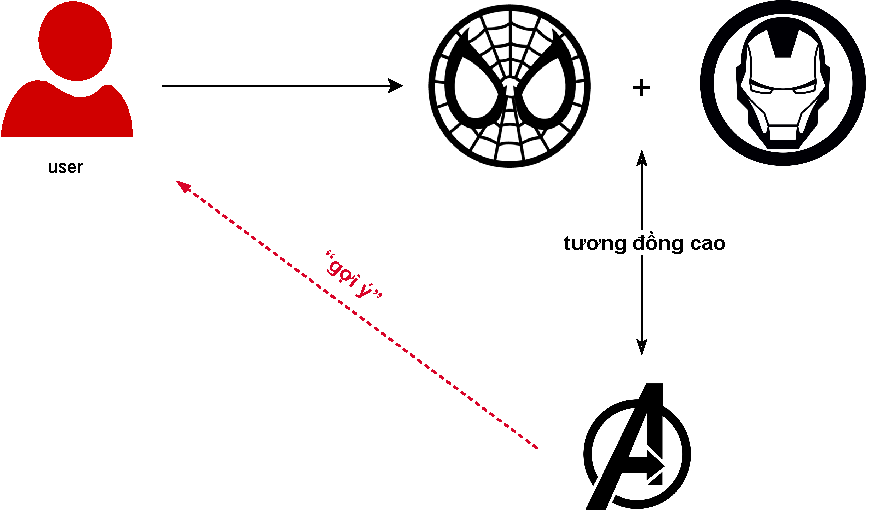
\includegraphics[width=0.6\textwidth]{CBF.pdf}
    \caption[Minh họa cách hoạt động của ``Content-Based Filtering'']{Minh họa cách hoạt động của ``Content-Based Filtering'':
    mô hình gợi ý bộ phim có độ tương đồng cao với các bộ phim
    người dùng đã xem trước đó}
    \label{fig_CBF}
\end{figure}
Hướng tiếp cận này làm cục bộ trong dữ liệu tương tác của mỗi người dùng và cần có thông tin mô tả của các sản phẩm, do đó nó có khả năng nắm bắt tốt các sở thích
đặc biệt của người dùng.
Vì dựa trên ``tính tương đồng'' của sản phẩm, hệ thống có thể gợi ý một sản phẩm phù hợp với người dùng nhưng sản phẩm này có thể không được nhiều người dùng khác quan tâm.
% Để áp dụng ``Content-Based Filtering'' cho từng loại dữ liệu cụ thể,
% ta cần ``domain knowledge'' cho lĩnh vực đó để thiết kế mô hình.
Nhược điểm của hướng tiếp cận ``Content-Based Filtering'' là cần phải có thông tin mô tả của các sản phẩm. Hơn nữa, từ thông tin mô tả sản phẩm, ta cũng cần đưa ra các đặc trưng mà sẽ giúp ích cho quá trình tính độ tương đồng của các sản phẩm; việc đưa ra các đặc trưng thường phụ thuộc vào lĩnh vực cụ thể và cần có hiểu biết về lĩnh vực đó (``domain knowledge'').

Một hướng tiếp cận khác là tìm ra ``độ tương đồng'' giữa các người dùng với nhau, hay tìm ra được các nhóm người dùng
có cùng sở thích dựa trên dữ liệu tương tác của tất cả người dùng. Khi đó, để có thể gợi ý cho một người dùng cụ thể,
hệ thống sẽ tìm ra các sản phẩm không có trong lịch sử tương tác của người dùng đó, và đã được những người dùng ``tương đồng'' với họ tương tác trước đó; hướng tiếp cận này được gọi là ``Collaborative Filtering'' (lọc cộng tác) (hình~\ref{fig_CF} mô tả hướng tiếp cận này).
\begin{figure}
    \centering
    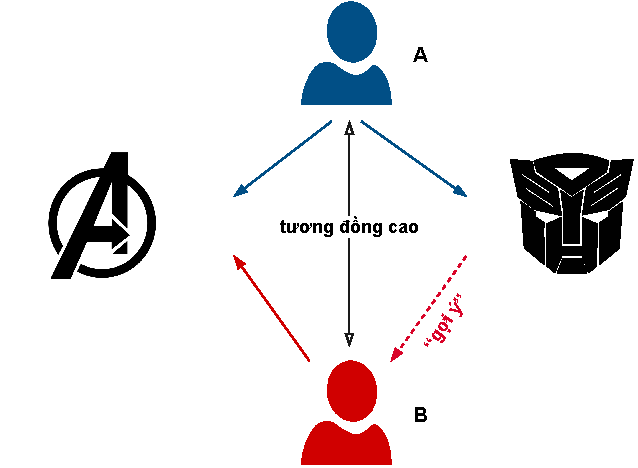
\includegraphics[width=0.6\textwidth]{CF.pdf}
    \caption[Minh họa cách hoạt động của ``Collaborative Filtering'']{Minh họa cách hoạt động của ``Collaborative Filtering'': hai người dùng cùng xem một (hoặc nhiều) bộ phim 
    sẽ được hệ thống đánh giá là hai người dùng ``tương đồng'' nhau, khi đó một bộ phim được
    người dùng A xem sẽ được gợi ý cho người dùng B}
    \label{fig_CF}
\end{figure}
Đối với hướng tiếp cận ``Collaborative Filtering'', mô hình dựa vào lịch sử tương tác từ người dùng khác
và không dùng các thuộc tính mô tả của sản phẩm, do đó nó có khả năng tạo ra sự tình cờ cho người dùng:
hệ thống có thể gợi ý một sản phẩm ``tốt'' cho người dùng trong trường hợp sản phẩm đó có ít điểm tương đồng
so với các sản phẩm người dùng đã ``thích'' trước đó. Hướng tiếp cận này chỉ cần dữ liệu đầu vào là các tương tác của các người dùng với các sản phẩm, do đó có thể áp dụng cho nhiều lĩnh vực khác nhau mà không cần thiết phải thay đổi cấu trúc hệ thống 
hoặc nếu có thì cũng không cần phải thay đổi quá nhiều.
Nhược điểm của ``Collaborative Filtering'' là cần dữ liệu tương tác của nhiều người dùng và mỗi người dùng cũng cần phải tương tác với khá nhiều sản phẩm. Việc gợi ý dựa trên các người dùng khác có thể là ưu điểm nhưng cũng có thể là nhược điểm của ``Collaborative Filtering'' trong trường hợp người dùng có sở thích rất khác biệt với số đông.
Một nhược điểm khác là các sản phẩm khi chỉ được một số rất ít người dùng tương tác, hệ thống gợi ý sản phẩm thường có xu hướng ít gợi ý những sản phẩm này đến các người dùng khác; vấn đề này gọi là ``cold-start''.
% Tuy nhiên, ``Collaborative Filtering'' gặp phải một vấn đề được gọi là ``khởi động nguội'' (``cold-start''),
% đó là khi mà một người dùng chưa có hoặc có ít tương tác thì hệ thống sẽ thường khó đưa ra được gợi ý ``tốt'' cho họ. ``Collaborative Filtering'' vẫn sẽ đưa ra gợi ý cho người dùng này tuy nhiên mức độ phù hợp đối với người dùng không cao, giảm khả năng thu hút khách hàng.
% Đối với ``Content-based Filtering'', việc gợi ý các sản phẩm liên quan đến sản phẩm đòi hỏi người dùng đã tương tác với một vài sản phẩm trước đó, dựa trên đó mới có thể tính độ tương đồng giữa sản phẩm để đưa ra gợi ý.

% ``Cold-start'' cũng là khi các sản phẩm chỉ được một số ít người dùng tương tác, các sản phẩm này sẽ ít được hệ thống gợi ý cho người dùng.

Trong giới hạn của khóa luận này, chúng tôi chỉ tập trung tìm hiểu về hướng tiếp cận ``Collaborative Filtering'' 
vì ba lý do chính là:
\begin{itemize}
\item ``Collaborative Filtering'' có thể áp dụng cho nhiều lĩnh vực khác nhau bởi đầu vào của mô hình là ma trận tương tác giữa người dùng và sản phẩm, khác với ``Content-Based Filtering'' cần thiết kế mô hình cụ thể cho từng lĩnh vực khác nhau.
\item Với số lượng lớn và cùng với sự đa dạng của các ``sản phẩm'' hiện nay, việc gợi ý các sản phẩm tương đồng với nhau dễ trở nên nhàm chán, thay vào đó ``Collaborative Filtering'' gợi ý sản phẩm dựa trên những người dùng khác, có thể tạo ra sự tình cờ cũng như đa dạng sản phẩm hơn, giúp các sản phẩm được gợi ý bớt nhàm chán.
\item Ngoài ra, khi số lượng người dùng trên mạng Internet càng ngày càng tăng nhanh, ``Collaborative Filtering'' 
sẽ có được nhiều lợi thế hơn khi có thể kết hợp dữ liệu tương tác của các người dùng khác để đưa ra gợi ý.
\end{itemize}

Việc kết hợp giữa thông tin tương tác từ người dùng khác và thông tin chi tiết của sản phẩm được gọi là hướng tiếp cận ``Hybrid'', đây là hướng tiếp cận kết hợp giữa ``Collaborative Filtering'' và ``Content-Based Filtering''.
Hướng tiếp này sẽ giúp một hệ thống gợi ý sản phẩm hoạt động hiệu quả hơn. Nhưng đây là một điều không đơn giản bởi nó phụ thuộc vào ``domain knowledge'' ở từng lĩnh vực và chúng tôi để lại như một định hướng trong việc nghiên cứu và phát triển trong tương tai.

Phương pháp đầu tiên trong việc xây dựng một hệ thống gợi ý sản phẩm theo hướng tiếp cận ``Collaborative Filtering'' là thuật toán ``Matrix Factorization'' được giới thiệu bởi Hu \cite{MF}. 
Ý tưởng là từ dữ liệu tương tác (ví dụ là số điểm đánh giá) của các người dùng với các sản phẩm, ta sẽ tìm ra các véc-tơ đặc trưng cho người dùng và các véc-tơ đặc trưng cho sản phẩm. 
Sau đó, ta sẽ dùng các véc-tơ đặc trưng này để dự đoán tương tác của người dùng với các sản phẩm mà họ chưa tương tác; từ kết quả dự đoán, ta sẽ đưa ra các đề xuất sản phẩm cho các người dùng.
Sau khi học và tìm ra được đặc trưng cho người dùng và sản phẩm trong tập huấn luyện, để đưa ra gợi ý cho người dùng mới, ta sẽ tìm véc-tơ đặc trưng ứng với người dùng mới và kết hợp với véc-tơ đặc trưng của sản phẩm để dự đoán được véc-tơ tương tác của người dùng mới này.
Dựa vào véc-tơ tương tác được dự đoán ta sẽ đưa ra gợi ý cho người dùng.
Cho đến hiện nay, ``Matrix Factorization'' vẫn  là một phương pháp đơn giản nhưng vẫn mang lại kết quả cao.
Tuy nhiên, thuật toán này có các nhược điểm mà khó có thể được áp dụng để xây dựng một hệ thống gợi ý sản phẩm quy mô lớn.
Đầu tiên, đó là số lượng tham số của mô hình tỉ lệ tuyến tính vào cả số lượng người dùng và số lượng sản phẩm. 
Ngày nay, số lượng người dùng và sản phẩm tăng rất nhanh theo thời gian, do đó số lượng tham số cũng như chi phí tính toán của mô hình là rất lớn.
Vì mô hình cần phải tìm ra các véc-tơ đặc trưng cho cả người dùng và sản phẩm, khi có người dùng mới, mô hình cần phải thực hiện một số bước tính toán để có thể tìm được đặc trưng của người dùng đó.
Ngoài ra, ``Matrix Factorization'' vẫn còn hạn chế đó là mô hình này là một mô hình tuyến tính, do đó nó chưa có khả năng ``học'' được các ``đặc trưng phi tuyến'' của dữ liệu.

``Asymetric Matrix Factorization'' là một phương pháp cải tiến từ ``Matrix Factorization''.
Với ý tưởng rút trích các đặc trưng của người dùng thông qua các sản phẩm mà họ đã tương tác, thay vì đặc trưng đến từ toàn bộ các sản phẩm trong hệ thống như ``Matrix Factorization''.
Phương pháp này đã khắc phục được nhược điểm của ``Matrix Factorization'' khi mà số lượng tham số của mô hình giờ chỉ phụ thuộc vào số lượng sản phẩm có trong hệ thống. 
Trong thực tế, số lượng sản phẩm sẽ tăng chậm hơn đáng kể so với số lượng người dùng trong hệ thống thì khắc phục này sẽ là một điểm mạnh của ``Asymetric Matrix Factorization''. 
Ngoài ra, mô hình này đã giảm bớt được chi phí tính toán để đưa ra dự đoán cho người dùng mới. 
Tuy nhiên, với hạn chế của các hàm tuyến tính nên phương pháp này vẫn chưa thực sự hiệu quả.

Ở công trình nghiên cứu [11] của tác giả Steck đã chỉ ra rằng “Asymetric Matrix Factorization” có thể được xem như là một mô hình “Auto-Encoder” tuyến tính. 
Cụ thể, mô hình ``Auto-Encoder'' tuyến tính này sẽ có véc-tơ đầu vào là véc-tơ chứa các tương tác của một người dùng với các sản phẩm (véc-tơ này sẽ có các giá trị thiếu ứng với các sản phẩm mà người dùng chưa tương tác). 
Véc-tơ đầu vào này sẽ đi qua bộ mã hóa của "Auto-Encoder" - là một hàm tuyến tính - để ra được véc-tơ đặc trưng của người dùng. 
Từ véc-tơ đặc trưng này, ``Auto-Encoder'' sẽ dùng bộ giải mã - là một hàm tuyến tính khác - để tái tạo lại véc-tơ đầu vào. 
Các tham số của bộ mã hóa và bộ giải mã sẽ được học từ dữ liệu tương tác của người dùng với các sản phẩm. 
Trong quá trình học, ta sẽ cố gắng tái tạo lại véc-tơ đầu vào nhưng không xét các giá trị thiếu. 
Miễn là các sản phẩm ứng với các giá trị thiếu của một véc-tơ đầu vào không bị thiếu trong các véc-tơ đầu vào khác thì ``Auto-Encoder'' vẫn sẽ có thể học được các tham số của bộ giải mã ứng với các sản phẩm này. 
Sau khi học xong, với véc-tơ đầu vào của một người dùng (có các giá trị thiếu), ta sẽ lan truyền qua bộ mã hóa và bộ giải mã của ``Auto-Encoder'' để có được véc-tơ đầu vào được tái tạo lại, trong đó các giá trị thiếu sẽ được điền giá trị. 
Từ các giá trị thiếu được điền này, ta có thể đưa ra các gợi ý sản phẩm cho người dùng. 
Từ mô hình ``Auto-Encoder'' tuyến tính, ta có thể dễ dàng mở rộng thành ``Auto-Encoder'' phi tuyến bằng cách thay các hàm tuyến tính ứng với bộ mã hóa và bộ giả mã bằng các hàm phi tuyến. 
Đây chính là ý tưởng của mô hình ``AutoRec'' được đề xuất trong bài báo \cite{autorec}. 
Đây là một trong những mô hình phi tuyến đầu tiên được đề xuất để giải quyết bài toán gợi ý sản phẩm. 
Tính phi tuyến đã giúp mô hình này đạt được kết quả tốt hơn so với các mô hình tuyến tính trên các bộ dữ liệu được bài báo thử nghiệm

% Dựa trên ý tưởng rằng, giả định tương tác của người dùng sẽ được ``phát sinh'' từ một ``đặc trưng ẩn'', ta có thể xem rằng ``đặc trưng ẩn'' này là sở thích của họ, và ta sẽ xây dựng một mô hình phát sinh được đặc trưng ẩn của người dùng từ dữ liệu tương tác của người dùng với hệ thống các sản phẩm. 
% Dựa trên ý tưởng là tồn tại các ``đặc trưng ẩn'' thể hiện sở thích của người dùng, các đặc trưng ẩn này sẽ dẫn đến người dùng ``tương tác'' với sản phẩm nào. Việc áp dụng mô hình ``Auto-Encoder'' hoàn toàn khớp với ý tưởng này, theo đó ``Auto-Encoder'' sẽ rút trích các ``đặc trưng ẩn'' này thông qua ``encoder'' (một phần trong mô hình ``Auto-Encoder''), sau đó tái tạo lại tương tác của người dùng dựa vào đặc trưng ẩn này. Tương tác được tái tạo lại sẽ bao gồm các gợi ý mà hệ thống đưa ra.

% Trong thời gian gần đây đã có nhiều nghiên cứu áp dụng mô hình ``Auto-Encoder'' trong bài toán xây dựng hệ thống gợi ý sản phẩm để có thể tận dụng sức mạnh của các hàm phi tuyến, cụ thể là sử dụng mạng nơ-ron với các hàm kích hoạt phi tuyến (là kiến trúc cơ bản của các mô hình được dùng huấn luyện trong lĩnh vực học máy) để có được một mô hình ``mạnh'' hơn so với các phương pháp tuyến tính trước đó.
% ``AutoRec'' \cite{autorec} được Sedhain giới thiệu tại hội nghị WWW2015, là mô hình được coi là đầu tiên trong việc sử dụng kiến trúc mô hình ``Auto-Encoder'' để đưa ra gợi ý cho người dùng bằng cách huấn luyện mô hình để tái tạo lại dữ liệu tương tác của người dùng sau khi trích xuất đặc trưng ẩn từ dữ liệu tương tác của họ.

Sau khi mô hình ``AutoRec'' được công bố, đã có nhiều công trình nghiên cứu đi theo hướng tiếp cận dùng "Auto-Encoder" phi tuyến để giải quyết bài toán gợi ý sản phẩm. 
``Collaborative denoising auto-encoders for top-n recommender systems'' \cite{cdae} (CDAE) được Wu cùng các cộng sự đề xuất nhằm hướng đến bài toán đưa ra gợi ý theo hướng xếp hạng và đưa ra ``top-N sản phẩm'' phù hợp nhất với người dùng hay nói cách khác là dự đoán tập các sản phẩm mà người dùng ``thích'' nhất. 
Mô hình này được xây dựng dựa trên ``AutoRec'' nhưng có các chỉnh sửa để phù hợp hơn với bài toán xây dựng hệ thống gợi ý sản phẩm khi mà ta quan tâm đến việc đưa ra xếp hạng các sản phẩm phù hợp với người dùng thay vì tái tạo lại tương tác của họ. 
Ngoài ra, trong quá trình học, với một véc-tơ đầu vào, mô hình này bỏ đi ngẫu nhiên một số phần tử (giống như bị thiếu giá trị) nhưng vẫn cố gắng tái tạo lại véc-tơ đầu vào mà không bỏ đi phần tử. 
Kỹ thuật này gọi là "denoising" (hay "drop-out") và giúp Auto-Encoder hoạt động tốt hơn với bài toán sản phẩm gợi ý sản phẩm, vì để đưa ra gợi ý sau khi học thì mô hình cần điền các giá trị thiếu của véc-tơ đầu vào.

% Ngoài ra, CDAE còn cải tiến từ ``AutoRec'' đó là thêm ``nhiễu'' vào dữ liệu huấn luyện nhằm giúp mô hình tránh được tình trạng ``Over-fitting'' (là trình trạng mà mô hình học ``tủ'' trên tập dữ liệu được huấn luyện nên mô hình đạt kết quả thấp trên các tập dữ liệu kiểm định), thường gặp phải khi huấn luyện mạng nơ-ron với hàm kích hoạt phi tuyến.
Tại hội nghị “International World Wide Web Conference Committee 2018”, các nhà nghiên cứu của Netflix-Google-MIT đã công bố bài báo "Variational Autoencoders for Collaborative Filtering", trong đó đề xuất mô hình mô hình "Variational Autoencoders" (VAE) cho bài toán gợi ý sản phẩm.
Ngoài việc tích hợp tất cả các ý tưởng đã được đề xuất trước đó (dùng hàm phi tuyến, dùng kỹ thuật "denoising" trong quá trình huấn luyện, hướng mô hình học được vào mục đích xếp hạng các sản phẩm), VAE giúp chống hiện tượng overfitting (hiện tượng "học tủ" trên tập huấn luyện nhưng dự đoán không tốt với dữ liệu ngoài tập huấn luyện) tốt hơn bằng cách: từ một véc-tơ đầu vào, VAE không tính ra một véc-tơ đặc trưng cố định như Auto-Encoder thông thường mà VAE ước lượng phân bố xác suất của véc-tơ đặc trưng (nghĩa là có sự không chắc chắn, và sự không chắc chắn này có thể giúp VAE chống được "overfitting"). 
Điều này giúp VAE đạt được kết quả tốt hơn so với các mô hình Auto-Encoder trước đó trên các tập dữ liệu được bài báo thử nghiệm. 
Trong một bài báo kiểm chứng tính hiệu quả của các mô hình phi tuyến so với các mô hình tuyến tính cho bài toán gợi ý sản phẩm [3], VAE là mô hình duy nhất được các tác giả kết luận là có hiệu quả so với các mô hình tuyến tính.

%----------------------Add in---------------------%
% Với một mô hình ``Auto-encoder'' nói chung, ta thường chỉ quan tâm đến việc thu được véc-tơ biểu diễn ẩn có thể hiện đúng tính chất của dữ liệu đầu vào sau quá trình huấn luyện. Ứng dụng của mô hình này thường là trích xuất các đặc trưng ẩn hoặc giảm chiều dữ liệu - đồng nghĩa với việc tái tạo dữ liệu là một quá trình phụ trợ cho việc huấn luyện mô hình. Nghĩa là mô hình sẽ tái tạo hoặc trích xuất được các ``đặc trưng ẩn'' của dữ liệu mà không thể sinh ra dữ liệu mới. 
% Ứng dụng của ``Auto-encoder'' trong các bài báo \cite{autorec,cdae} trong hệ thống gợi ý là cố gắng tái tạo lại ``đặc trưng ẩn của người dùng'', từ đó cũng sinh ra các gợi ý.
% Vô tình, ý tưởng này dẫn đến rằng việc đưa ra gợi ý không phải là mục đích chính của mô hình, mà gợi ý được tạo một cách gián tiếp thông qua việc tái tạo lại dữ liệu.
% Với bài toán xây dựng hệ thống gợi ý, việc tạo ra các gợi ý cho người dùng phải là một việc được ưu tiên. 
% Mô hình VAE với ``đặc trưng ẩn'' được phát sinh từ một phân phối xác suất, và được xem như một mô hình có thể phát sinh dữ liệu mới từ ``đặc trưng ẩn''. 
% Khi ứng dụng trong bài toán xây dựng hệ thống gợi ý, việc phát sinh dữ liệu mới này tương đồng với việc tạo ra các gợi ý, đồng thời cũng vẫn giữ được tính chất của ``Auto-encoder'' trong bài toán này là tương tác người dùng được phát sinh từ một ``đặc trưng ẩn'' (cũng chính là thể hiện cho sở thích của người dùng).


Với nền tảng của mô hình VAE dựa trên phương pháp ``Variational Inference'' trong lĩnh vực xác suất thống kê. 
``Variational Inference'' dùng để suy diễn dữ liệu ẩn từ dữ liệu ta quan sát được, hay cụ thể trong bài toán này là suy diễn các ``đặc trưng ẩn'' dựa vào dữ liệu quan sát được là các tương tác của người dùng. 
Đặc điểm của phương pháp này là có thể áp dụng tốt cho dữ liệu thưa, có nghĩa là đối với ``dữ liệu quan sát được'' bị hạn chế thì việc ``suy diễn'' dữ liệu vẫn đạt được kết quả tốt. 
Dữ liệu thưa là dữ liệu mà đa phần các phần tử trong một điểm dữ liệu mang giá trị 0.
Trong hệ thống gợi ý, tính chất của dữ liệu thường là thưa do mỗi người dùng chỉ tương tác với một lượng nhỏ sản phẩm trên toàn hệ thống, từ đó việc suy diễn trở nên hiệu quả trong hệ thống gợi ý.

Mục tiêu sau cùng của hệ thống gợi ý sản phẩm đó là tập sản phẩm được gợi ý sẽ phù hợp nhất đối với người dùng. 
Do đó, trong tập sản phẩm này thì cũng cần phải được sắp xếp theo thứ tự giảm dần theo thứ tự giảm dần về độ phù hợp.
Để kết quả trả về từ mô hình có thể đạt được mục tiêu trên thì tác giả Liang đã giới thiệu ``Multinomial log-likelihood'' cho việc tính toán độ lỗi. 
Với tính chất trả về một giá trị xác suất cho mỗi sản phẩm, và tổng giá trị xác suất trên toàn bộ sản phẩm là 1. 
Các sản phẩm sẽ phải ``cạnh tranh'' với nhau để có được xác suất cao hơn.

Với những gì đã trình bày ở trên, trong khóa luận, chúng tôi sẽ tập trung tìm hiểu về mô hình VAE cho bài toán gợi ý sản phẩm \cite{mvae}. 
Chúng tôi sẽ cài đặt lại mô hình này và so sánh kết quả cài đặt của chúng tôi với kết quả của bài báo gốc.
Ngoài ra, chúng tôi sẽ tiến hành thêm các thí nghiệm nhằm phân tích rõ hơn về các khía cạnh khác nhau của mô hình này


%--------------------------------------------------%

% Lý do đầu tiên mà chúng tôi quyết định tìm hiểu về mô hình này cũng như là điểm khác biệt của VAE so với các phương pháp đã được kể đến ở trên đó là đặc trưng ẩn được phát sinh là một phân phối xác suất thay vì là ``một điểm dữ liệu cố định'' (``Auto-Encoder'' và ``Denosing Auto-Encoder'' sẽ nhận dữ liệu đầu vào ở chiều không gian ``cao'' và trích xuất đặc trưng ẩn là một điểm dữ liệu ở chiều không gian ``thấp'' hơn mà vẫn thể thể hiện được ``tính chất'' của dữ liệu ban đầu).
% Việc đặc trưng ẩn là một phân phối xuất sẽ giúp cho mô hình có thể sử dụng dặc trưng ẩn này để phát sinh dữ liệu, ứng dụng với bài toán ta đang quan tâm đó chính là sử dụng sở thích nắm bắt được từ các người dùng để đưa ra gợi ý cho họ.
% Nền tảng của VAE đó là dựa trên phương pháp ``Variational Inference'', một phương pháp trong lĩnh vực xác suất thống kê. 
% Phương pháp này thường được dùng để suy diễn ``dữ liệu ẩn'' dựa trên những ``dữ liệu ta quan sát được''. Đặc điểm của phương pháp này là có thể áp dụng tốt cho dữ liệu thưa, có nghĩa là đối với ``dữ liệu quan sát'' được bị hạn chế thì việc ``suy diễn'' dữ liệu vẫn đạt được kết quả tốt. 
% Ở đây, trong bài toán xây dựng hệ thống gợi ý sản phẩm, dữ liệu tương tác của người dùng sẽ được xem là dữ liệu quan sát được và đặc trưng ẩn là ``dữ liệu ẩn'' mà ta không quan sát được. 
% Đặc biệt ở đây, đối với bài toán xây dựng hệ thống gợi ý sản phẩm thì thông thường mỗi người dùng chỉ tương tác với một lượng tỉ lệ nhỏ các sản phẩm so với toàn bộ sản phẩm có trong hệ thống, do đó việc áp dụng phương pháp ``Variational Inference'' hay nói cách khác là VAE sẽ phù hợp với bài toán xây dựng hệ thống gợi ý sản phẩm dựa trên ý tưởng phát sinh tương tác của người dựa vào đặc trưng ẩn của người dùng.
% Bên cạnh đó, để có thể xây dựng một mô hình giải quyết giải quyết vấn đề mà hệ thống gợi ý sản phẩm quan tâm đó là có thể đưa ra được tập các sản phẩm có khả năng cao sẽ phù hợp với người dùng, mục đích này khác hoàn toàn với việc tái tạo lại dữ liệu hay nói cách khác là tái tạo lại tương tác của người dùng.
% Với mục tiêu để mô hình thể hiện được rõ khả năng mà một sản phẩm có phù hợp với người dùng hay không thì tác giả Liang đã sử dụng hàm ``Multinomial log-likelihood'' (một phương pháp đánh giá bộ tham số của mô hình với giả định dữ liệu tương tác của người dùng tuân theo một phân phối đa thức). 
% ``Multinomial log-likelihood'' sẽ khiến kết quả trả về từ mô hình thể hiện ``giá trị độ lớn về xác suất''. Với ``multinomial log-likelihood'' các sản phẩm sẽ phải ``cạnh tranh'' với nhau để có thể đạt được xác suất được chọn cao hơn (vì kết quả trả về sẽ phải ràng buộc là tổng kết quả  ``xác suất'' trả về sẽ bằng 1 hay xác suất được chọn của các sản phẩm trả về từ mô hình sẽ có tổng bằng 1).
% Tuy không được sử dụng nhiều trong lĩnh vực xây dựng hệ thống gợi ý sản phẩm, thay vào đó, ``Multinomial log-likelihood'' lại thường được sử dụng nhiều trong các lĩnh vực về mô hình ngôn ngữ (Language models) hay về các bài toán trong lĩnh vực kinh tế (Ecomomics) nhưng chúng tôi tin rằng ``Multinomial log-likelihood'' sẽ là một lựa chọn phù hợp trong lĩnh vực xây dựng hệ thống gợi ý sản phẩm.

% Cuối cùng, một điểm đặc biệt của phương pháp này đó là tác giả đã đề xuất thêm một siêu tham số để kiểm soát việc đánh đổi giữa việc tối thiểu độ lỗi trong việc mô hình hóa dữ liệu và việc đảm bảo đặc trưng ẩn được phát sinh tuân theo phân phối xác suất được giả định từ mô hình. 
% Siêu tham số là một tham số được chỉ định bởi lập trình viên cho mô hình thay vì mô hình học phải học như các tham số thông thường.
% Nguyên nhân dẫn đến việc cần phải có một siêu tham số để kiểm soát được việc đánh đổi nói trên là vì với việc xây dựng một hệ thống gợi ý sản phẩm thì chúng ta sẽ quan tâm tới việc mô hình hoá dữ liệu nhiều hơn là việc đảm bảo đặc trưng ẩn sẽ tuân theo phân phối xác suất. 
% Nói một cách khác, thì việc mô hình hoá dữ liệu sẽ đảm bảo rằng đặc trưng ẩn có được từ mô hình sẽ thể hiện được cho dữ liệu ban đầu, hay trong bài toán xây dựng hệ thống gợi ý thì điều này đảm bảo mô hình sẽ nắm bắt được xu hướng sở thích giữa các người dùng nhưng nếu mô hình chỉ tập trung để mô hình hoá dữ liệu thì mô hình sẽ bị giới hạn lại thành việc tái tạo lại tương tác của người dùng.
% Còn về việc đảm bảo tính chất về phân phối xác suất sẽ giúp cho đặc trưng có thể phát sinh được dữ liệu một cách hợp lý, nếu quá tập trung để đảm bảo điều này thì mô hình sẽ khó nắm  bắt được sở thích chung giữa các người dùng, ngược lại, nếu bỏ qua tính chất này, thì đặc trưng ẩn sẽ khó có thể đưa ra được những sản phẩm không nằm trong lịch sử tương tác mà phù hợp với người dùng.
% Do vậy, khi xây dựng hệ thống gợi ý sản phảm thì ta sẽ cần phải kiểm soát được việc đánh đổi này thì hệ thống gợi ý mới có thể hoạt động hiệu quả hơn.

% Mặc dù không phải là mô hình đạt được kết quả tốt nhất hiện nay trong việc xây dựng hệ thống gợi ý sản phẩm, tuy 
% nhiên kiến thức nền tảng để xây dựng mô hình này bao phủ về lĩnh vực học máy cũng như là kiến thức về mô hình xác suất.
% Với những lợi điểm như trên, thì chúng tôi đã quyết định sẽ tập trung tìm hiểu mô hình được tác giả Liang đề xuất ở bài báo \cite{mvae}. 


% Tuy có những lợi điểm trên nhưng trong thực tế thì để VAE có thể ``hoạt động'' tốt với bài toán xây dựng hệ thống gợi ý sản phẩm thì không dễ.
% Để VAE ``hoạt động'', có hai việc cần phải giải quyết là: (i) kết quả trả về từ mô hình sẽ là tập các sản phẩm được dự đoán là có khả năng thể hiện sự phù hợp với người dùng chứ việc tái tạo lại dữ liệu ban đầu không phải mục tiêu chính trong việc xây dựng hệ thống gợi ý sản phẩm và (ii) đánh đổi giữa việc tái tạo lại dữ liệu và việc đặc trưng ẩn được phát sinh tuân theo giả định về phân phối xác suất của mô hình.
% Để kết quả trả về từ mô hình là tập các sản phẩm có ``xác suất'' hay thể hiện sự phù hợp với người dùng thì chúng tôi sử dụng hàm 
% % ``Multinomial log-likelihood'' (hàm log-likelihood là hàm số dùng để đánh giá bộ trọng số của mô hình), 
% ``Multinomial log-likelihood'' (một phương pháp đánh giá bộ tham số của mô hình với giả định dữ liệu tương tác của người dùng tuân theo một phân phối đa thức),
% ``Multinomial log-likelihood'' sẽ khiến kết quả trả về từ mô hình thể hiện ``giá trị độ lớn về xác suất''. Với ``multinomial log-likelihood'' các sản phẩm sẽ phải ``cạnh tranh'' với nhau để có thể đạt được xác suất được chọn cao hơn (vì kết quả trả về sẽ phải ràng buộc là tổng kết quả  ``xác suất'' trả về sẽ bằng 1 hay xác suất được chọn của các sản phẩm trả về từ mô hình sẽ có tổng bằng 1).
% Tuy không được sử dụng nhiều trong lĩnh vực xây dựng hệ thống gợi ý sản phẩm, thay vào đó, ``multinomial log-likelihood'' lại thường được sử dụng nhiều trong các lĩnh vực về mô hình ngôn ngữ (Language models) hay về các bài toán trong lĩnh vực kinh tế (Ecomomics) nhưng chúng tôi tin rằng ``multinomial log-likelihood'' sẽ là một lựa chọn phù hợp trong lĩnh vực xây dựng hệ thống gợi ý sản phẩm.
% Về vấn đề đánh đổi giữa việc tối thiểu độ lỗi trong việc mô hình hóa dữ liệu và việc đảm bảo đặc trưng ẩn được phát sinh tuân theo phân phối xác suất được giả định từ mô hình thì chúng tôi sử dụng một siêu tham số mới để kiểm soát việc đánh đổi này.
% Tuy nhiên, với việc sử dụng siêu tham số để kiểm soát về việc đánh đổi nói trên thì ta sẽ cần phải giải quyết thêm một vấn đề khác đó là việc lựa chọn siêu tham số phù hợp cho mô hình. Siêu tham số là một tham số được chỉ định bởi lập trình viên cho mô hình thay vì mô hình học phải học như các tham số thông thường.
% Thường thì việc lựa chọn siêu tham số cho các mô hình học là một công đoạn tốn thời gian và phiền phức khi mà ta cần phải chạy mô hình nhiều lần với các bộ siêu tham số khác nhau để chọn ra được siêu tham số để mô hình có kết quả tốt.
% Như vậy, có hai câu hỏi được trả lời để mở rộng VAE cho bài toán xây dựng hệ thống gợi ý sản phẩm là: (i) tại sao Multinomial log-likelihood lại phù hợp hơn với bài toán xây dựng hệ thống gợi ý sản phẩm?; (ii) làm sao để tối ưu được việc đánh đổi giữa độ lỗi trong việc mô hình hoá dữ liệu và việc đảm bảo đặc trưng ẩn có được từ mô hình tuân theo một phân phối xác suất được giả định. Cụ thể:
% \begin{itemize}
%     \item Chúng tôi tiến thành thực hiện huấn luyện mô hình VAE với hàm ``multinomial log-likelihood'' và chúng tôi gọi VAE với hàm ``multinomial log-likelihood'' là Mult-VAE. Bên cạnh đó, chúng tôi cũng thực hiện huấn luyện VAE để so sánh hàm log-likelihood này với các hàm log-likelihood thường được áp dụng khi huấn luyện VAE là Gaussian log-likelihood và Logistic likelihood.
%     \item Hơn nữa, chúng tôi cũng đề xuất một siêu tham số để kiểm soát việc đánh đổi thường gặp khi huấn luyện VAE. Và phương pháp để lựa chọn cho siêu tham số này thay vì phải thực hiện huấn luyện với các gía trị siêu tham số khác nhau.
% \end{itemize}

% Với hai thành phần trên (sử dụng hàm multinomal log-likelighood và siêu tham sô kiểm soát sự đánh đổi trong lúc huấn luyện), kết quả thí nghiệm trên các bộ dữ liệu lớn trong tác vụ xây dựng hệ thống gợi ý sản phẩm như Movielens-20M và Million Song Datasets cho thấy Mult-VAE đạt được kết quả ấn tượng, ngoài ra việc sử dụng hàm multinomial log-likelihood cho kết quả tốt hơn so với các hàm log-likelihood thông dụng khác.


Phần còn lại của khóa luận được trình bày như sau:

\begin{itemize}
    \item Chương~\ref{Chapter2} trình bày sơ lược về mô hình ``Auto-Encoder'' và các kiến thức nền tảng của mô hình ``Variational Auto-Encoder''.
    % \item Chương~\ref{Chapter3} trình bày về cách áp dụng mô hình ``Variational Auto-Encoder'' cùng với hàm lỗi ``Multinomial log-likelihood'' cho bài toán xây dựng hệ thống gợi ý. Bên cạnh đó, chương này cũng phân tích các hạn chế của mô hình đồng thời đề xuất phương pháp giúp giải quyết các hạn chế đó. Chương này là phần chính của khóa luận.
    \item Chương~\ref{Chapter3} trình bày về mô hình được đề xuất ở bài báo \cite{mvae}. Đầu tiên, chúng tôi sẽ trình bày cách áp dụng mô hình ``Auto-Encoder'' để xây dựng một hệ thống gợi ý sản phẩm ở mức cơ bản. Kế tiếp, chúng tôi trình bày những hạn chế của mô hình này và dẫn dắt đến mô hình ``Variational Auto-Encoder'' cùng với một số tinh chỉnh để có được hệ thống gợi ý sản phẩm tốt hơn. Chương này là phần chính của khóa luận.  
    \item Chương~\ref{Chapter4} trình bày về các thí nghiệm và các kết quả đạt được.
    \item Cuối cùng, tổng kết và hướng phát triển được trình bày ở chương~\ref{Chapter5}.
\end{itemize}

